% VERSTERKER

    In dit verslag wordt het designproces van hoogfrequente single-stage
    versterker besproken die gerealiseerd wordt in common emitter-opstelling.

    Hierbij is de gebruikte NPN-transistor een BFR91A en werd
    het werkingspunt in \cite{lesWendy} gespecificeerd zoals weergegeven in
    \autoref{tbl:OPSpec}.
      \begin{table}[h!]
        \begin{center}

        \caption{DC werkingspunt transistor}
        \label{tbl:OPSpec}
        
 \begin{tabular}{|l|l|l|l|} 
\hline \textbf{Groep} & \textbf{Frequentie $f_0$} & \textbf{$V_{ce}$} & \textbf{$I_c$}\\ 
\hline $1$ & $1445$ MHz & $5$ V & $5$ mA \\ 
\hline \end{tabular} 

        \end{center}
      \end{table} 
    
    Voor deze werkingsfrequentie werden de $S$-parameters gegeven in \cite{lesWendy}:
    \[
S = \left[ \begin{array}{cc} 
S_{11} & S_{12} \\ 
 S_{21} & S_{22} \\ 
\end{array} \right] 
 \approx \left[ \begin{array}{cc} 
-0.104 +0.181 j & 0.102 +0.154 j \\ 
1.369 +1.397 j & 0.355 -0.318 j \\ 
\end{array} \right] \label{eq:S}
\]
    
\section{Stabiliteit}
    We controleren de nodige en voldoende voorwaarde voor stabiliteit van de versterker
    door middel van formules 11.71 en 11.72 van \cite{Pozar}.
    Dit is het Rollet-stabiliteitscriterium.
    \[
      K = \frac{1 - \left| S_{11} \right|^2 - \left| S_{22} \right|^2 + \left| \Delta \right|^2}{2 \left| S_{12}S_{21} \right|} > 1
    \]
    \[
      \left| \Delta \right| < 1
    \]
    \[
      \Delta = \det{S} = S_{11}S_{22} - S_{12}S_{21}
    \]
    Numeriek geeft dit:
    \[
K \approx 1.113 \qquad \qquad 
|\Delta| \approx |0.096 -0.256j| \approx 0.273 
\]

    Aan de stabiliteitsvoorwaarden is voldaan, zodat men kan besluiten dat de te
    realiseren versterker onconditioneel stabiel is.
  \section{Stabiliteitscirkels}
    Vermits de versterker onconditioneel stabiel is, zullen de stabiliteitscirkels
    ofwel de volledige Smith Chart omvatten ofwel buiten de Smith Chart vallen.
    Toch wordt dit nogmaals gecontroleerd.

    De stabiliteitscirkels geven de reflectiefactoren (en dus ook de matching-
    impedanties) aan waarvoor de hele schakeling nog net stabiel is voor de
    opgegeven werkingsfrequentie. Onvoorwaardelijke stabiliteit zegt dus enkel
    dat indien de versterker voorzien wordt van passieve netwerken aan de in-
    en uitgang dat er geen oscillator op de werkingsfrequentie gemaakt is.
    Wat echter niet aangetoond wordt met dit stabiliteitscriterium is de
    afwezigheid van oscillaties op andere frequenties!
    
    Met formules 11.68 en 11.69 uit \cite{Pozar}, worden middelpunt $C$ en
    straal $R$ van de stabiliteitscirkels bepaald.
    \[
      C_L = \frac{\conj{\left(S_{22} - \Delta \conj{S_{11}}\right)}}{\left| S_{22} \right|^2 - \left|\Delta\right|^2}
      \qquad \qquad \qquad
      R_L = \left| \frac{S_{12}S_{21}}{\left| S_{22} \right|^2 - \left|\Delta\right|^2}\right|
    \]
    \[
      C_S = \frac{\conj{\left(S_{11} - \Delta \conj{S_{22}}\right)}}{\left| S_{11} \right|^2 - \left|\Delta\right|^2}
      \qquad \qquad \qquad
      R_S = \left| \frac{S_{12}S_{21}}{\left| S_{11} \right|^2 - \left|\Delta\right|^2}\right|
    \]
    Dit geeft aanleiding tot volgende waarden:
    \[
	C_L =	  2.70 + j   2.15\qquad \qquad \qquad  	R_L =	  2.37
\]

    \[
	C_S =	  7.04  +7.73 j\qquad \qquad \qquad	R_S =	 11.58
\]

    Op \autoref{fig:stabCirkels} kunnen deze cirkels ge\"inspecteerd worden.
    \begin{figure}[!h]
      \centering
      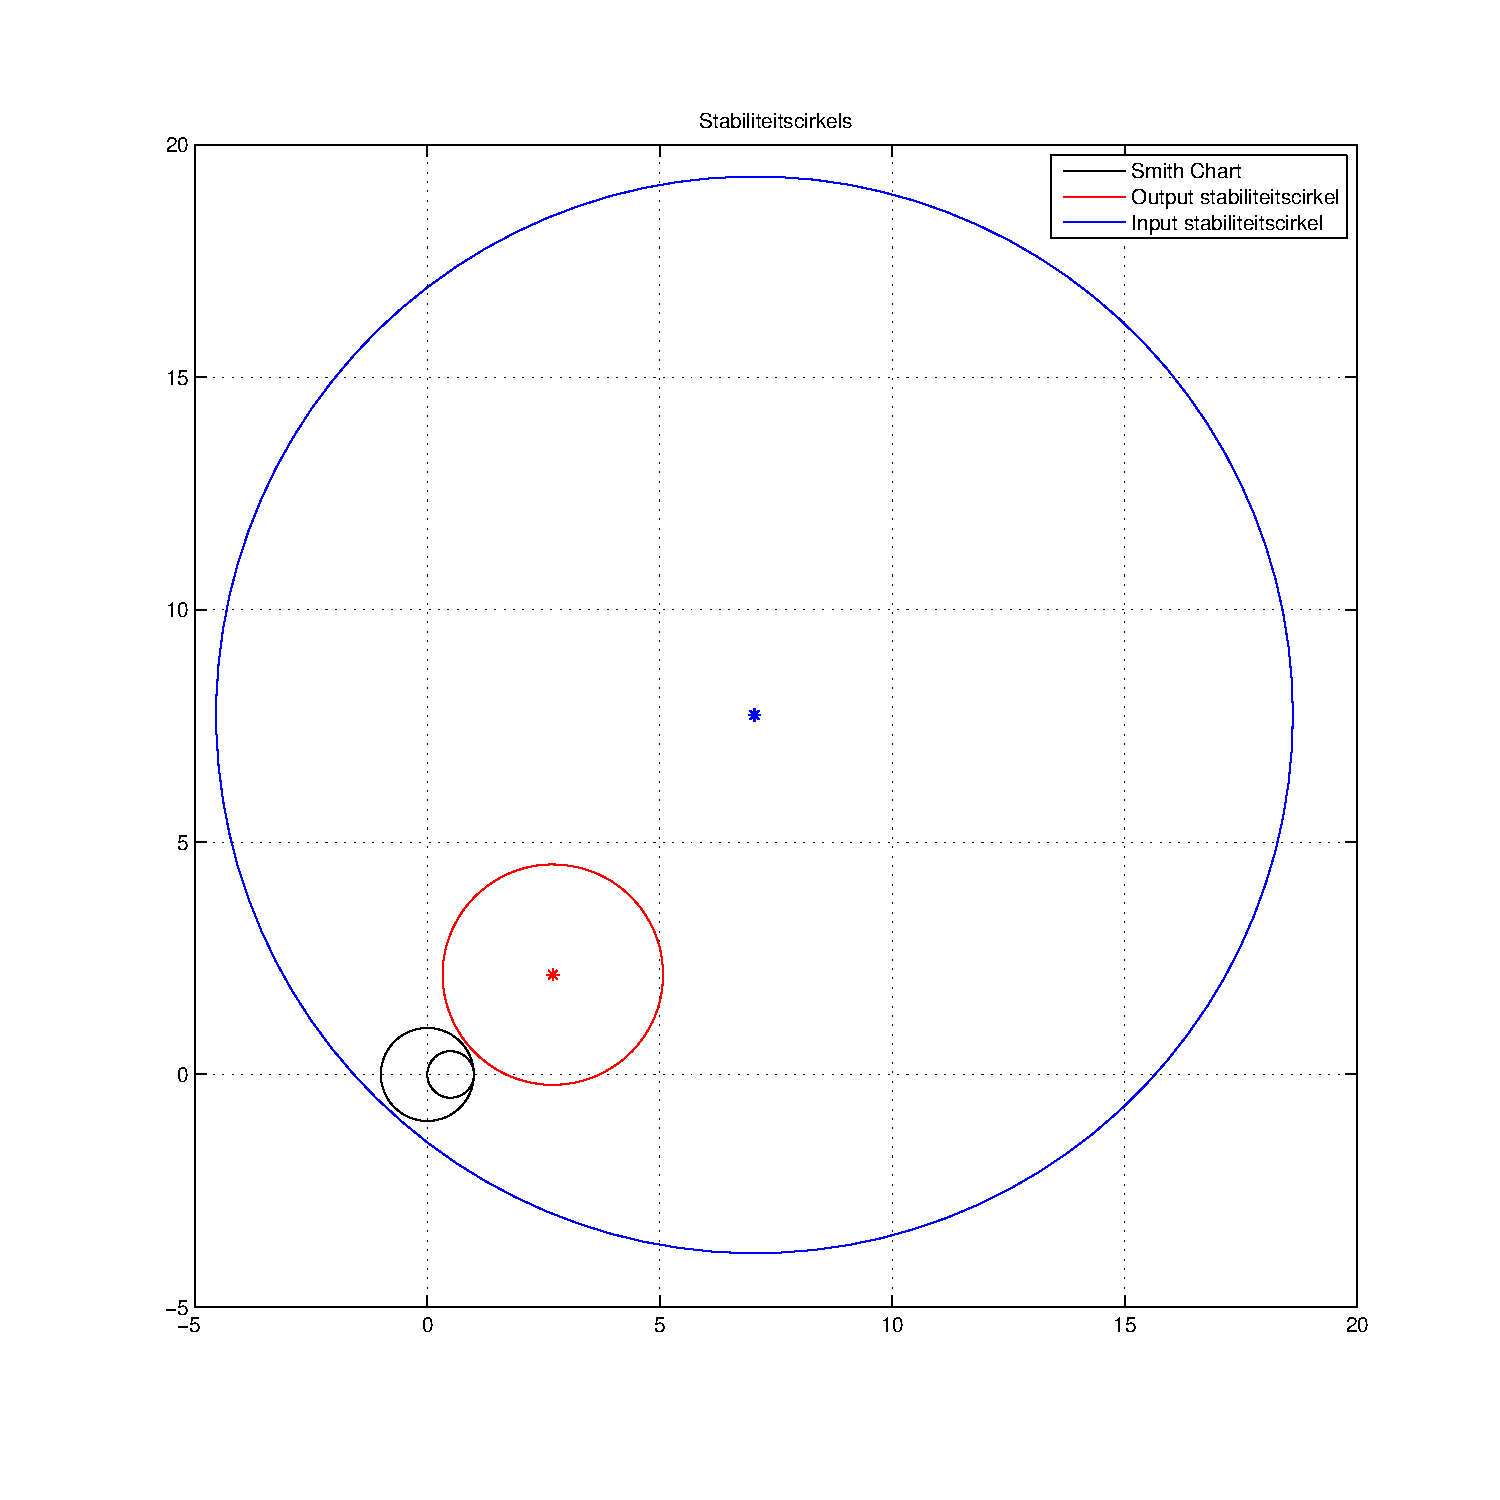
\includegraphics[width=\textwidth,keepaspectratio=true]{fig/stabiliteitscirkels.pdf}  
      \caption{Stabiliteitscirkels} 
      \label{fig:stabCirkels}
    \end{figure}
    Als extra controle, bekijken we welke zones van de Smith Chart stabiel zijn voor input en output. We volgen hier
    een analoge redenering als beschreven op pagina 614 van \cite{Pozar}.
    
    \paragraph{Voor de input} weten we dat indien de output perfect gematcht is
    ($Z_L = Z_0$ en dus ook $\Gamma_L = 0$, oftewel in het midden van de Smith
    Chart), we formule 11.62a uit \cite{Pozar}
    \[
      \left| \Gamma_{in} \right| = \left| S_{11} + \frac{S_{12}S_{21}\Gamma_L}{1 - S_{22}\Gamma_L} \right| < 1
    \]
    kunnen vereenvoudigen tot:
    \[
      \left| S_{11} \right|  < 1
    \]
    als voorwaarde voor stabiliteit. Hieraan is voldaan zoals we kunnen zien uit
    de S-parameters van de transistor. Hierdoor weten we dat het gebied binnen
    de blauwe inputsstabiliteitcirkel stabiel is.
    
    \paragraph{Voor de output} volgt analoog dat indien de input perfect
    gematcht is ($Z_S = Z_0$ en dus ook $\Gamma_S = 0$, oftewel in het
    midden van de Smith Chart), we formule 11.62b uit \cite{Pozar}
    \[
      \left| \Gamma_{out} \right| = \left| S_{22} + \frac{S_{12}S_{21}\Gamma_S}{1 - S_{11}\Gamma_S} \right| < 1
    \]
    kunnen vereenvoudigen tot:
    \[
      \left| S_{22} \right|  < 1
    \]
    als voorwaarde voor stabiliteit. Hieraan is voldaan zoals we kunnen zien uit
    de S-parameters van de transistor. Hierdoor weten we dat het gebied buiten
    de rode outputsstabiliteitcirkel stabiel is.
    

\section{Gebruik van de unilaterale benadering}
  Als verantwoording voor de unilaterale benadering, gebruiken we formule 11.86
  uit \cite{Pozar} die slechts enkele tienden van een dB afwijking mag geven.
  We nemen hiervoor de grenswaarde van $0.8 dB$
  \[
    -0.8 dB < \frac{1}{\left( 1 + U\right)^ 2} < \frac{G_T}{G_{TU}} < \frac{1}{\left( 1 - U\right)^ 2} < 0.8 dB
  \]
  In deze formule is $U$ de \textit{unilateral figure of merit}:
  \[
    U = \frac{\norm{S_{12}} \norm{S_{21}} \norm{S_{11}} \norm{S_{22}}}{ \left( 1 - \norm{S_{11}}^2 \right) \left( 1 - \norm{S_{22}}^2 \right)}
  \]
  In numerieke waarden, geven deze vergelijkingen dus:
    \[
	U \approx	0.04863
\]
\[
-0.8 \,dB < 0.90940 < \frac{G_T}{G_{TU}} < 1.10484 < 0.8 \,dB
\]
\[
-0.8 dB < -0.825 \,dB< \frac{G_T}{G_{TU}} < 0.866 \,dB< 0.8 \,dB
\]

  Vermits deze ongelijkheden geldig zijn, mag de unilaterale benadering gebruikt
  worden.
  
  

\section{Berekening van maximale versterking}
  Aan de hand van \cite{Pozar} en \cite{Gonzalez} wordt de maximale transducergain
  op de gegeven werkingsfrequentie bepaald.
  
  In appendix E van \cite{Gonzalez} werd bewezen dat bovenstaande uitdrukking
  voor een onconditioneel stabiele transistor (K > 1) en simultane input- en
  outputmatching, de maximale versterking uitgedukt
  kan worden als:
  \[
    G_{Tmax} = \frac{\norm{S_{21}}}{\norm{S_{12}}} \left( K - \sqrt{K^2-1}\right)
  \]
  
  
  \section{Bepaling van de constante gaincirkels}
  Uit formules 5.96 en 5.100 van \cite{lessen} kan men het middelpunt en de
  straal van de constante gaincirkels voor gain $G_p$ bepalen.
  \[
    C = \frac{\left( \conj{S_{22}} - S_{11} \conj{\Delta} \right)}{\norm{S_{22}}^2 - \norm{\Delta}^2 + \frac{\norm{S_{21}}^ 2}{G_p}}
  \]
  \[
    R = \frac{\sqrt{\norm{S_{12} S_{21}}^2 - 2 K \norm{S_{12} S_{21} \frac{\norm{S_{21}}^2}{G_p} + \frac{\norm{S_{21}}^2}{G_p} }}}{\norm{S_{22}}^2 - \norm{\Delta}^2 + \frac{\norm{S_{21}}^2}{G_p}}
  \]
  Voor een versterking van enkele verschillende versterkingen $G_p$ bekomt men
  in deze formule de waarden weergegeven in \autoref{tbl:gainCirkels}.
    \begin{table}[h!]
    \begin{center}
    \caption{Constante gaincirkels}
    \label{tbl:gainCirkels}
    \begin{tabular}{|r|r|r|} \hline 
\textbf{Versterking $G_p$} & \textbf{Middelpunt $C$} & \textbf{Straal $R$} \\ \hline 
$ 3.000$ \mbox{dB} & $ 0.111 -0.127 j$ &  0.804 \\ \hline 
$ 2.000$ \mbox{dB} & $ 0.100 -0.113 j$ &  0.824 \\ \hline 
$ 1.000$ \mbox{dB} & $ 0.089 -0.102 j$ &  0.843 \\ \hline 
$10.390$ \mbox{dB} & $ 0.243 -0.277 j$ &  0.561 \\ \hline 
$16.323$ \mbox{dB} & $ 0.433 -0.492 j$ &  0.062 \\ \hline 
$16.411$ \mbox{dB} & $ 0.436 -0.495 j$ &  0.000 \\ \hline 
\end{tabular}
    \end{center}
    \end{table}
  
  Op de Smith Chart \cite{smithchart} in \autoref{fig:gainCirkels} worden deze
  constante gain cirkels voor enkele verschillende
  versterkingen weergegeven op.
  \begin{figure}[!h]
      \centering
      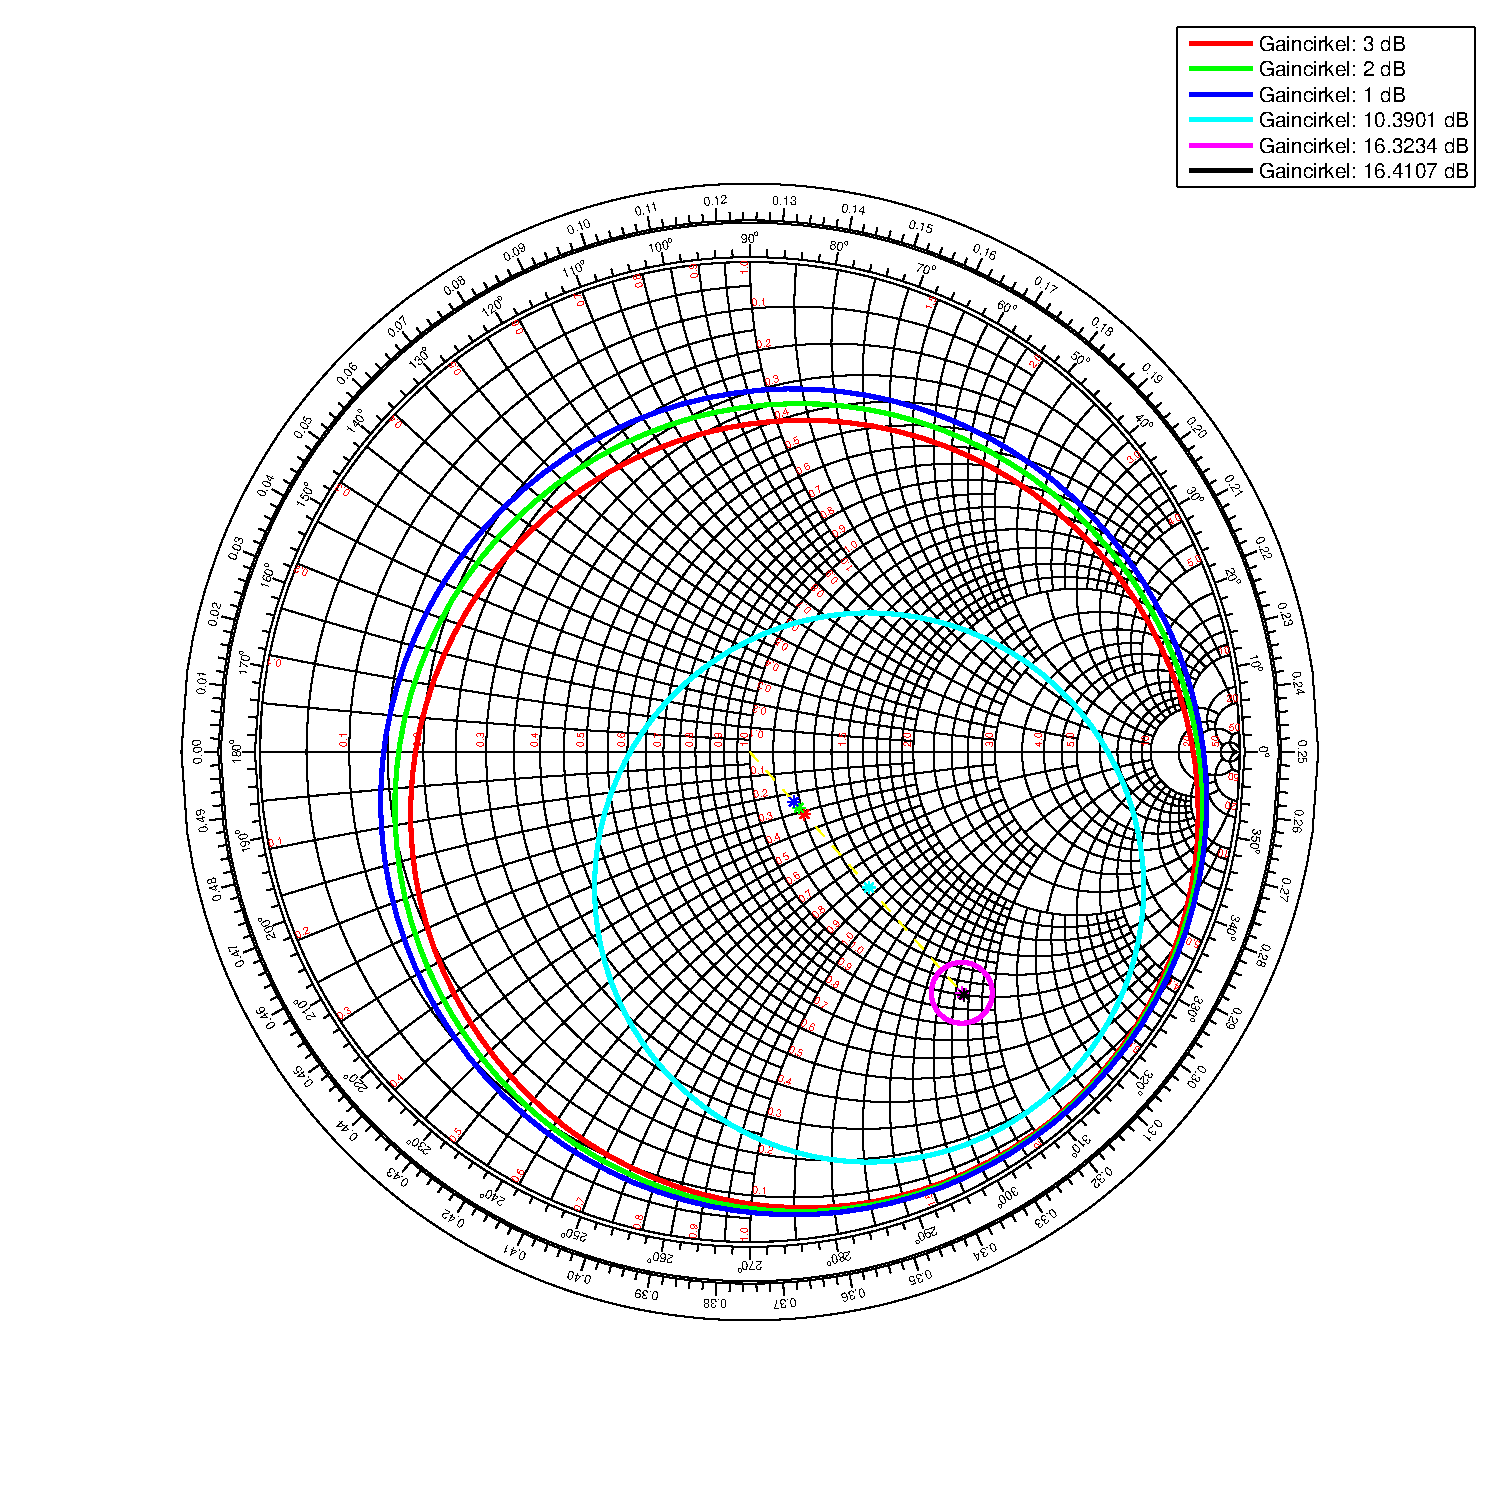
\includegraphics[width=\textwidth,keepaspectratio=true]{fig/gaincirkels.pdf}  
      \caption{Constante gaincirkels} 
      \label{fig:gainCirkels}
    \end{figure}
  

\section{Matchingnetwerken}

  \subsection{Bepalen van de te matchen reflectiefactoren}
    \tbd{Uitleg en formules bijsmijten}
  \subsection{De eigenlijke matching}
  Zoals opgelegd in \cite{lesWendy} wordt gebruikgemaakt van een variatie op de
  single stub matching zoals weergegeven in figuur \ref{fig:schakelingMatch}.
  De aangeduide impedantiepijlen dragen een nummer dat ook verder gebruikt zal
  worden als index bij de matching voor zowel reflectiefactoren ($\Gamma$),
  impedanties ($Z$), admittanties ($Y$), enz. Het is dus raadzaam deze schakeling bij de
  hand te houden. 

  \begin{figure}[!hb]
    \centering
    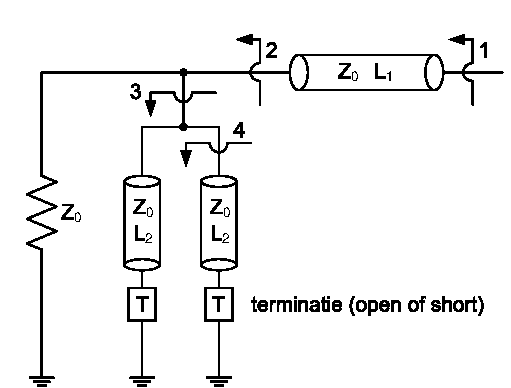
\includegraphics[keepaspectratio=true]{fig/matching.pdf}
    \caption{Schakeling matchingnetwerken}
    \label{fig:schakelingMatch}
  \end{figure}

  De matching gebeurt zowel voor ingang als uitgang gelijkaardig, vandaar ook
  dat er gekozen is om dit via MATLAB te implementeren in de functie \texttt{matcher}.

  Voor de ingang en uitgang kunnen de bijhorende smith charts op respectievelijk
  figuur \ref{fig:matchIn} en figuur \ref{fig:matchOut} gevolgd worden, dit
  zijn admittantie-smith charts genormaliseerd op $50 \Omega$. Deze zijn
  tevens in de bijlagen aanwezig voor de duidelijkheid. Verder in de tekst
  zal voor de beknoptheid gesproken worden over genormaliseerde conductanties
  en admittanties zonder dit expliciet te vermelden (bij niet-genormaliseerde
  grootheden worden echter steeds eenheden vermeld).

  Hier zal enkel algemeen de uitleg gegeven worden bij zowel de schakeling en de smith charts, zonder in
  detail te gaan voor in- of uitgang. In tabel \ref{tbl:Matching} wordt eveneens
  een korte legende voor de gebruikte Smith Charts weergegeven.

  \paragraph{N.B.} Vermits er enkel een impedantie smith chart beschikbaar is
  en men bij een match met parallele stubs het handiger is om met admittanties
  te werken, kunnen reflectiefactoren $\Gamma$ niet rechtstreeks uitgezet worden.
  Door $-\Gamma$ op de chart te noteren, is in feite een puntspiegeling rond de
  oorsprong gerealiseerd. Hierdoor zijn de isoweerstand- en isoreactantielijnen
  van de (getekende) impedantie smith chart, samenvallend met de isoconductantie-
  en isopermeantielijnen van de (denkbeeldige) admittantie smith chart.

  Bij het aflezen van reflectiefactoren moet echter wel steeds opnieuw de
  puntspiegeling uitgevoerd worden om de werkelijke reflectiefactoren te bekomen.
  Hiermee werd in wat hierop volgt steeds rekening gehouden.

  Dit houdt bv. ook in dat op de smith charts gebruikt voor de matchings, de
  open ($Z = \infty$, $Y=0$, $\Gamma = 1$) helemaal links ligt en de short
  ($Z = 0$, $Y = \infty$, $\Gamma = -1$) helemaal rechts.

  \begin{enumerate}
   \item Men zet eerst de vereiste reflectiefactor $\Gamma_1$ uit op de Smith
   Chart, deze werden op het einde van de vorige sectie bepaald.
   \item Vervolgens kan men (als hulpmiddel) een cirkel met als middelpunt $\varrho = 0 + 0j$ door
   het punt $\Gamma_1$ tekenen (in streep-punt-lijn), dit zijn alle realiseerbare
   reflectie-factoren $\gamma_2$ voor het punt $2$ als de tussenliggende
   transmissielijn verlies- en dispersieloos is.
   \item Men bepaalt vervolgens de twee snijpunten tussen de cirkel $\gamma_2$
   en de cirkel met conductantie $G = 1$. Voor allebei de snijpunten
   bepaalt men de hoek (of lengte) waarover naar load gedraaid (tegenwijzerzin)
   moet worden om vanuit $\Gamma_1$ in het snijpunt uit te komen.
   \item Het snijpunt met de kortste lengte, noemen we $\Gamma_2$ en de bijhorende
   lengte wordt aangeduidt met $L_1$ of in elektrische lengte $E_1$. Hiermee is
   de lengte van de eerste transmissielijn bepaald.
   \item Op het knooppunt $2$, kunnen we een verband tussen de admittanties opschrijven
   en vereenvoudigen vermits $\Re{(Y_2)} = 1$ per constructie.
   \[
     Y_2 = Y_3 + Y_0 = Y_3 \Rightarrow Y_3 = Y_2 - 1 = Y_2
   \]
   \item \tbd{Controle: er klopt echt iets niet: waarom complex toegevoegde nemen?}
   \item Hiermee hebben we $Y_3$ bepaald, en vermits $Y_3 = 2 \cdot Y_4$,
   is daaruit $\Gamma_4 = \frac{1-Y_4}{1+Y_4}$ te bepalen en uit te zetten
   op de smith chart.
   \item Vanuit $\Gamma_4$ draait men weer naar load (over de transmissielijn)
   tot men in de open of de short terechtgekomen is en leest men de lengte
   $L_2$ (elektrische lengte $E_2$) van de stublijn af.   
  \end{enumerate}


  De numerieke resultaten van deze matchings wordt weergegeven in tabel \ref{tbl:Matching}.

  \begin{figure}
    \centering
    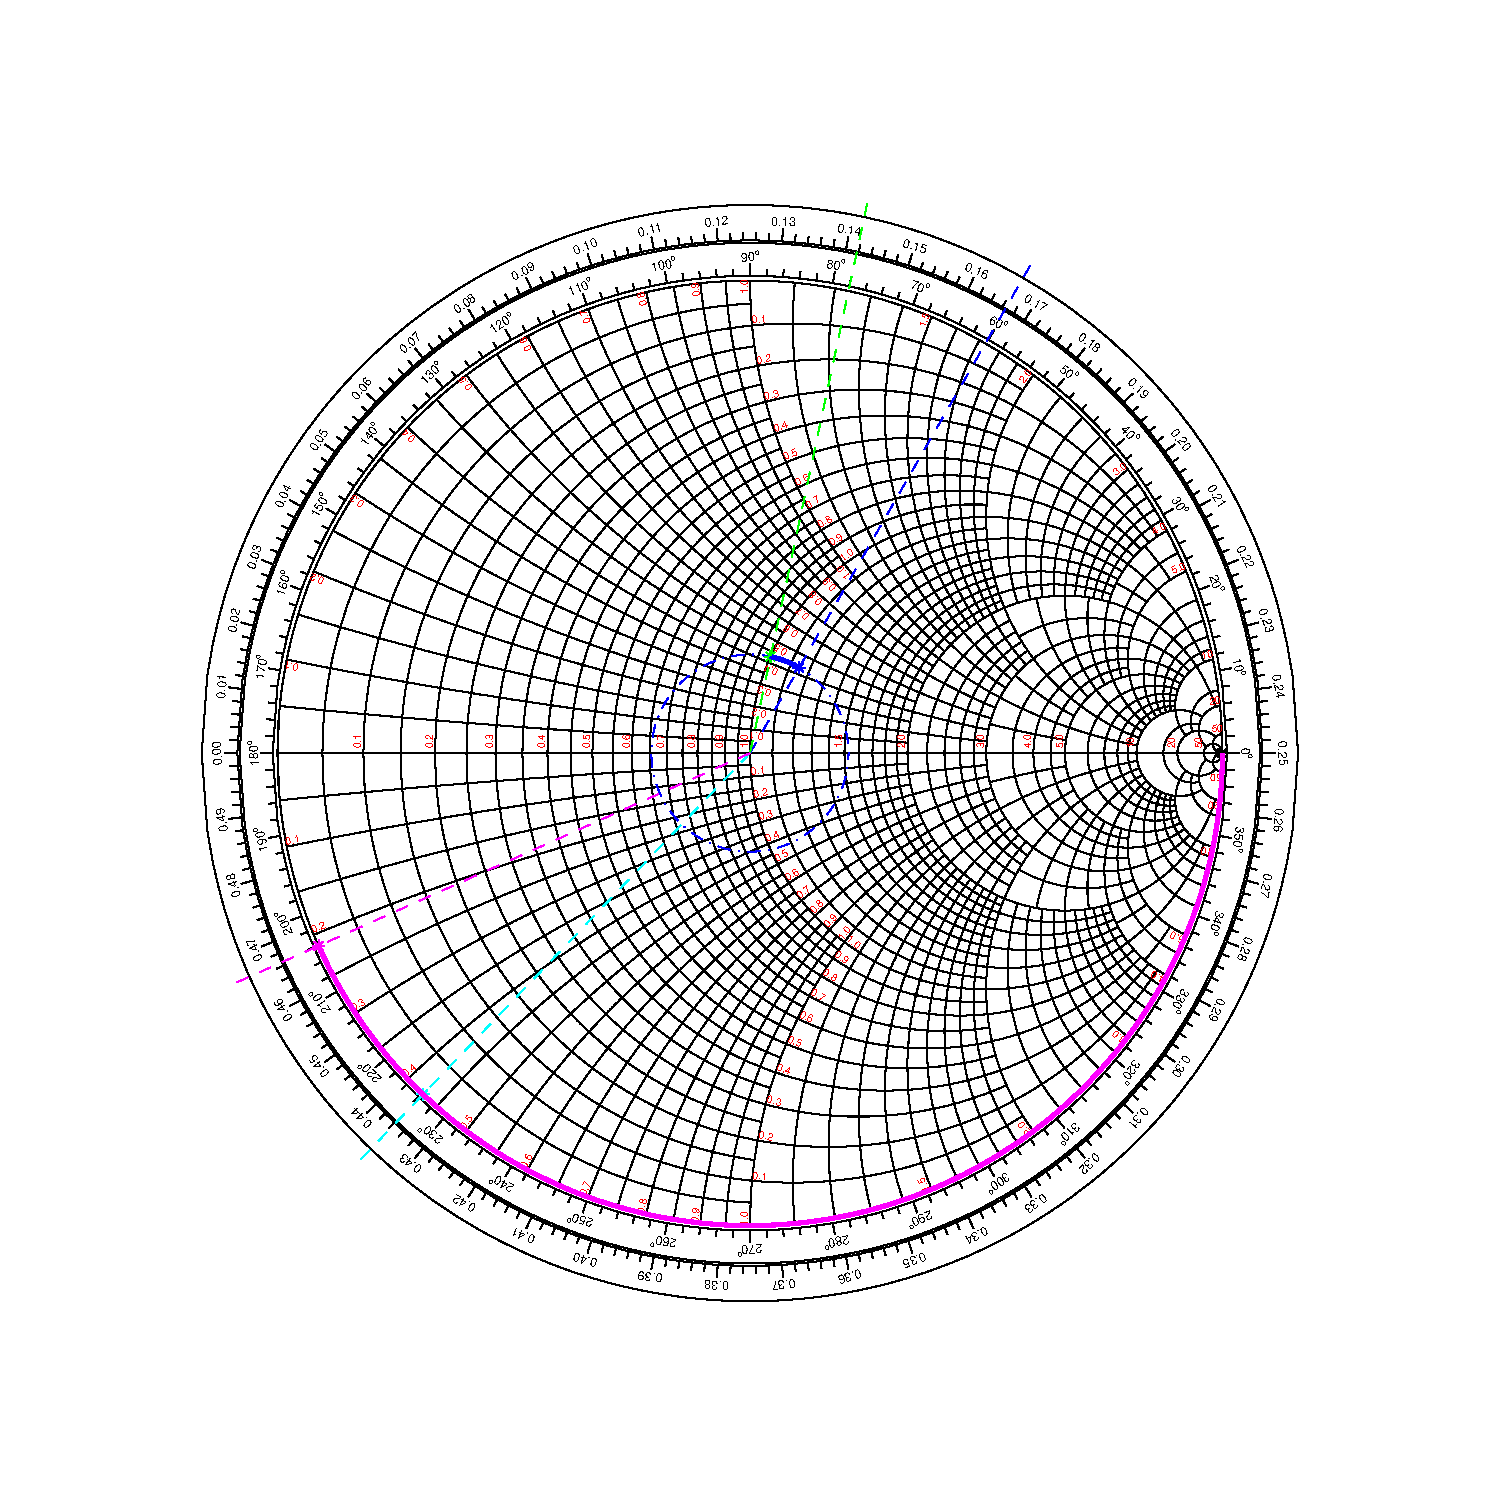
\includegraphics[width=\textwidth,keepaspectratio=true]{fig/matchSource.pdf}
    \caption{Smith Chart matchingnetwerk aan de ingang}
    \label{fig:matchIn}
  \end{figure}

  \begin{figure}
    \centering
    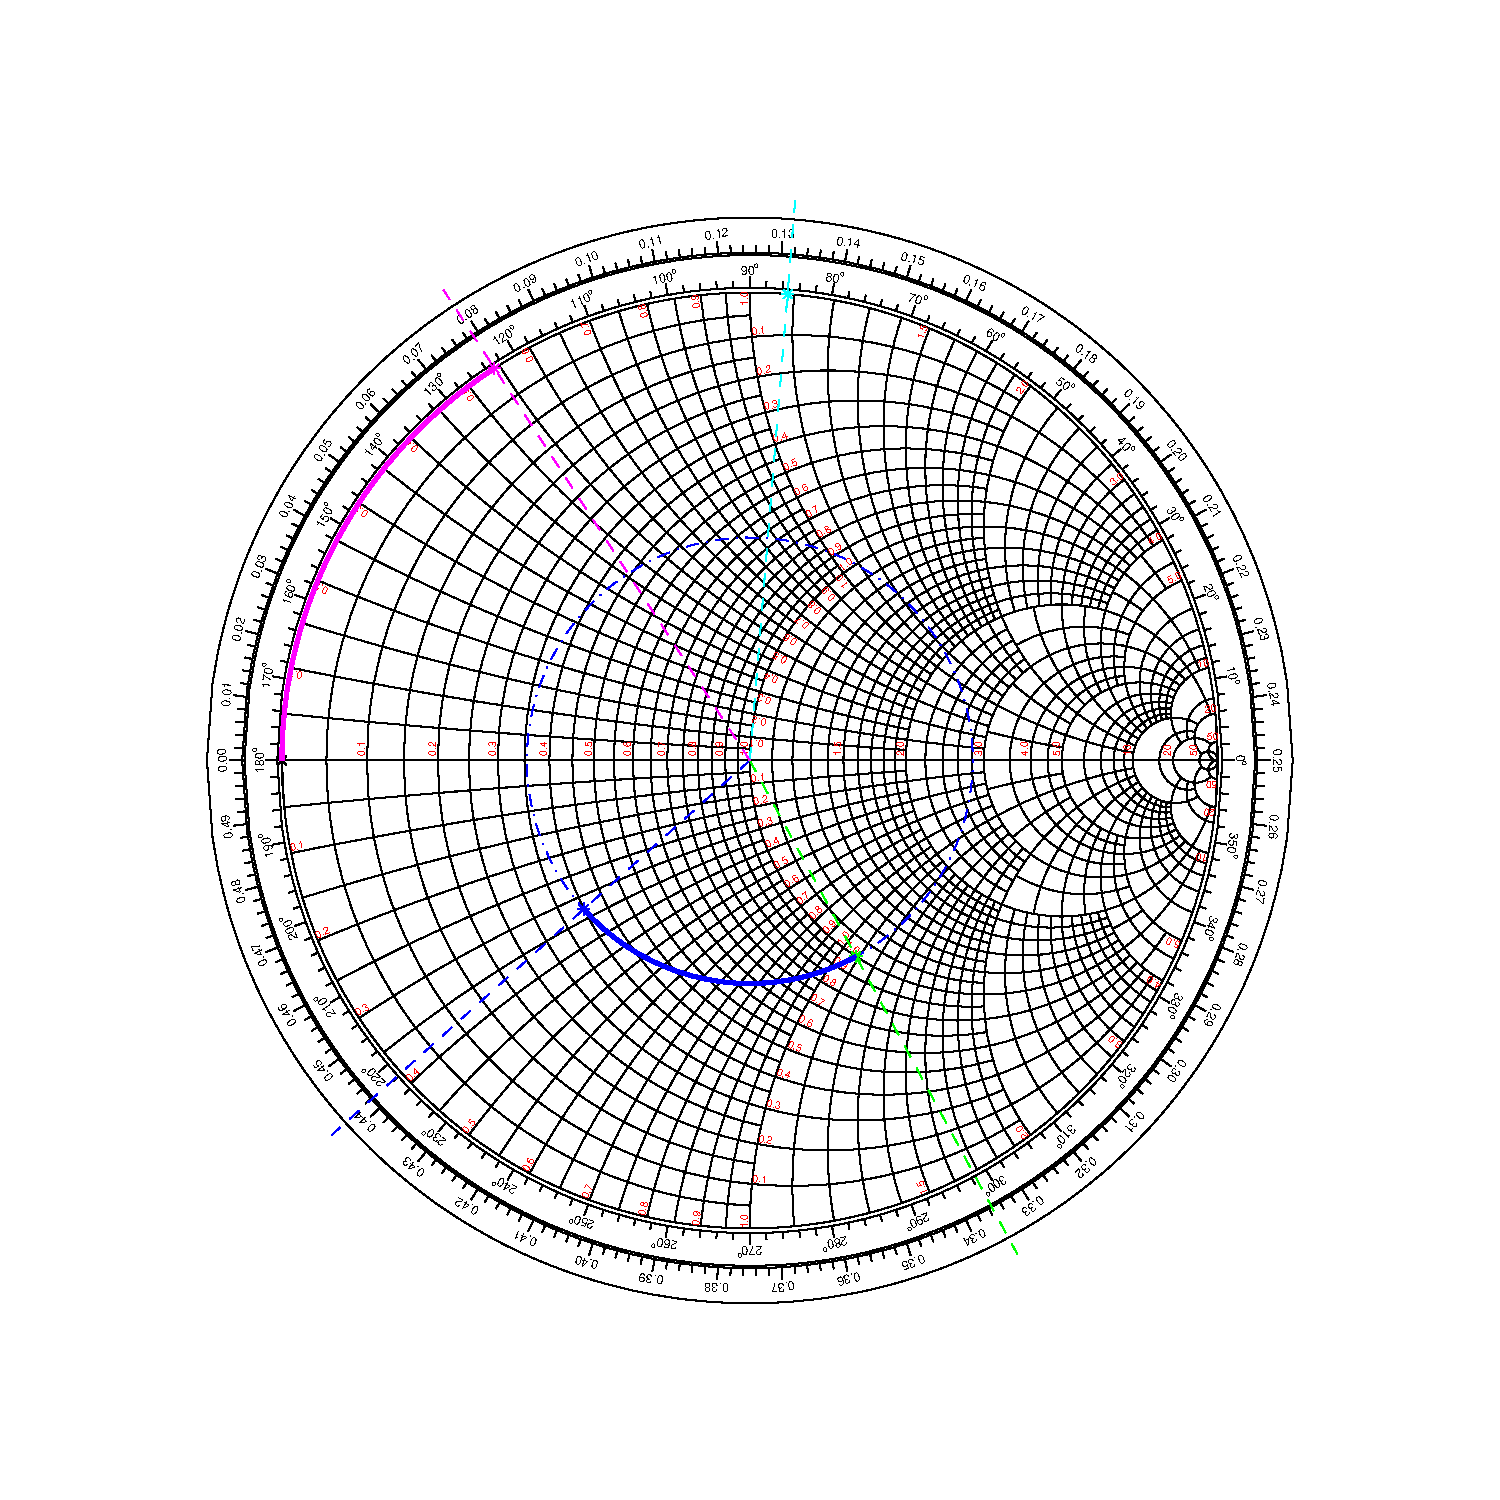
\includegraphics[width=\textwidth,keepaspectratio=true]{fig/matchLoad.pdf}
    \caption{Smith Chart matchingnetwerk aan de uitgang}
    \label{fig:matchOut}
  \end{figure}
  


  \begin{table}[h!]
     \begin{center}
       \caption{Matchingnetwerken}
       \label{tbl:Matching}
       \begin{tabular}{|lc|r|r|c|} 
\hline \textbf{Grootheid} & & \textbf{Ingang} & \textbf{Uitgang} & \\ 
\hline $\Gamma_1$ &  & $-0.401 -0.441 j$ & $0.563 +0.448 j$ &  \\ 
\hline $\Gamma_2$ &  & $0.355 -0.479 j$ & $0.517 +0.500 j$ &  \\ 
\hline $Y_2$ &  & $1.000 -1.485 j$ & $1.000 +2.071 j$ & S \\ 
\hline $\Gamma_3$ &  & $0.376 +0.927 j$ & $0.622 -0.783 j$ &  \\ 
\hline $Y_3$ &  & $-1.485 j$ & $+2.071 j$ & S \\ 
\hline $\Gamma_4$ &  & $-0.289 +0.957 j$ & $0.035 -0.999 j$ &  \\ 
\hline $Y_4$ &  & $-0.743 j$ & $+1.035 j$ & S \\ 
\hline $E_1$ &  & 78.896 & 5.500 & $^{\circ}$ \\ 
\hline $E_2$ &  & 73.201 & 88.005 & $^{\circ}$ \\ 
\hline terminatie &  & short & open &  \\ 
\hline \end{tabular} 

     \end{center}
  \end{table}


\section{DC biasnetwerk}
  Om het DC Bias-netwerk te designen kunnen vele verschillende soorten
  netwerken gebruikt worden. Hier werd de aanpak op pagina 275 uit \cite{Gonzalez}
  gebruikt. Volgens deze bron is dit netwerk (figuur \ref{fig:DCBias} aangepast
  bij het gebruik van (dunne en dikke) filmweerstanden, waarvan bij deze realisatie
  gebruik zal gemaakt worden.

  \begin{figure}
    \centering
    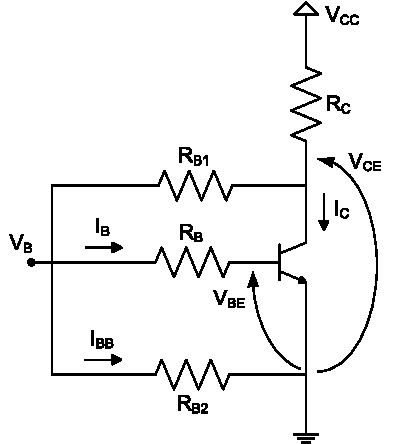
\includegraphics[keepaspectratio=true]{fig/DCBias.pdf}
    \label{fig:DCBias}
    \caption{Biasnetwerk}
  \end{figure}

  Om de componentwaarden te bepalen, maken we gebruik van de vergelijkingen uit
  \cite{Gonzalez}, die ook eenvoudig afgeleid zouden kunnen worden uit de
  werkingsvergelijkingen van een bipolaire transistor en algemenere
  netwerkvergelijkingen.
    \[
      I_B = \frac{I_C}{h_{FE}}
    \]
    \[
      R_B = \frac{V_B - V_{BE}}{I_B}
    \]
    \[
      R_{B2} = \frac{V_B}{I_{BB}}
    \]
    \[
      R_{B1} = \frac{V_{CE} - V_B}{I_{BB} + I_B}
    \]
  Bijkomend wordt gesteld dat om een goede stabiliteit van het biasnetwerk te
  bekomen, men erop moet letten dat $I_{BB} >> I_B$ en $V_{B} \approx 0.1 V_{CC}$.
  Vermits het werkingspunt in \cite{lesWendy} werd opgegeven zoals te zien in
  tabel \ref{tbl:OPSpec}. Uit \cite{BFR91A} kan de nominale waarde van de
  versterkingsfactor $h_{FE} \approx 100$ gehaald worden en het voor een
  siliciumtransistor is $V_{BE} \approx 0.7 \mbox{V}$.

  

\section{Simulaties}
  \subsection{Ideale transmissielijnen}
  \subsection{Microstrip}

\section{Lay-out}

\section{Metingen}
\subsection{Vergelijking metingen en simulaties}




\tbd{\textbf{Voor het verslag:}
  \begin{itemize}
    \item Alle berekeningen + verwijzing formule
    \item Plots van ideale simulaties + simulatie in microstripversie
    \item Gebruikte Smith Charts voor matching van in- en uitgang
  \end{itemize}
  }